\documentclass[a4paper,10pt]{article}
\usepackage[brazilian]{babel}
\usepackage[left=2.5cm,right=2.5cm,top=3cm,bottom=2.5cm]{geometry}
\usepackage{mathtools}
\usepackage{amsthm}
\usepackage{amsmath}
%\usepackage{nccmath}
\usepackage{amssymb}
\usepackage{amsfonts}
\usepackage{physics}
%\usepackage{dsfont}
%\usepackage{mathrsfs}

\usepackage{titling}
\usepackage{indentfirst}

\usepackage{bm}
\usepackage[dvipsnames]{xcolor}
\usepackage{cancel}

\usepackage{xurl}
\usepackage[colorlinks=true]{hyperref}

\usepackage{float}
\usepackage{graphicx}
%\usepackage{tikz}
\usepackage{caption}
\usepackage{subcaption}

%%%%%%%%%%%%%%%%%%%%%%%%%%%%%%%%%%%%%%%%%%%%%%%%%%%

\newcommand{\eps}{\epsilon}
\newcommand{\vphi}{\varphi}
\newcommand{\cte}{\text{cte}}

\newcommand{\N}{\mathbb{N}}
\newcommand{\Z}{\mathbb{Z}}
\newcommand{\Q}{\mathbb{Q}}
\newcommand{\R}{\vb{R}}
\newcommand{\C}{\mathbb{C}}
\renewcommand{\S}{\hat{S}}
%\renewcommand{\H}{\s{H}}

\renewcommand{\a}{\vb{a}}
\newcommand{\nn}{\hat{n}}
\renewcommand{\d}{\dagger}
\newcommand{\up}{\uparrow}
\newcommand{\down}{\downarrow}

\newcommand{\0}{\vb{0}}
%\newcommand{\1}{\mathds{1}}
\newcommand{\E}{\vb{E}}
\newcommand{\B}{\vb{B}}
\renewcommand{\v}{\vb{v}}
\renewcommand{\r}{\vb{r}}
\renewcommand{\k}{\vb{k}}
\newcommand{\p}{\vb{p}}
\newcommand{\q}{\vb{q}}
\newcommand{\F}{\vb{F}}

\newcommand{\s}{\sigma}
%\newcommand{\prodint}[2]{\left\langle #1 , #2 \right\rangle}
\newcommand{\cc}[1]{\overline{#1}}
\newcommand{\Eval}[3]{\eval{\left( #1 \right)}_{#2}^{#3}}

\newcommand{\unit}[1]{\; \mathrm{#1}}

\newcommand{\n}{\medskip}
\newcommand{\e}{\quad \mathrm{e} \quad}
\newcommand{\ou}{\quad \mathrm{ou} \quad}
\newcommand{\virg}{\, , \;}
\newcommand{\ptodo}{\forall \,}
\renewcommand{\implies}{\; \Rightarrow \;}
%\newcommand{\eqname}[1]{\tag*{#1}} % Tag equation with name

\setlength{\droptitle}{-7em}

\theoremstyle{plain}
\newtheorem{theorem}{Teorema}[section]
%\newtheorem{defi}[theorem]{Definição}
\newtheorem{lemma}[theorem]{Lema}
%\newtheorem{corol}[theorem]{Corolário}
%\newtheorem{prop}[theorem]{Proposição}
%\newtheorem{example}{Exemplo}
%
%\newtheorem{inneraxiom}{Axioma}
%\newenvironment{axioma}[1]
%  {\renewcommand\theinneraxiom{#1}\inneraxiom}
%  {\endinneraxiom}
%
%\newtheorem{innerpostulado}{Postulado}
%\newenvironment{postulado}[1]
%  {\renewcommand\theinnerpostulado{#1}\innerpostulado}
%  {\endinnerpostulado}
%
%\newtheorem{innerexercise}{Exercício}
%\newenvironment{exercise}[1]
%  {\renewcommand\theinnerexercise{#1}\innerexercise}
%  {\endinnerexercise}
%
%\newtheorem{innerthm}{Teorema}
%\newenvironment{teorema}[1]
%  {\renewcommand\theinnerthm{#1}\innerthm}
%  {\endinnerthm}
%
\newtheorem{innerlema}{Lema}
\newenvironment{lema}[1]
  {\renewcommand\theinnerlema{#1}\innerlema}
  {\endinnerlema}
%
%\theoremstyle{remark}
%\newtheorem*{hint}{Dica}
%\newtheorem*{notation}{Notação}
%\newtheorem*{obs}{Observação}


\title{\Huge{\textbf{Teoria de grupos - Exercício 1}}}
\author{Mateus Marques}

\begin{document}

\maketitle

\section*{Grupo da molécula de amônia NH$_3$}

\begin{figure}[H]
\centering
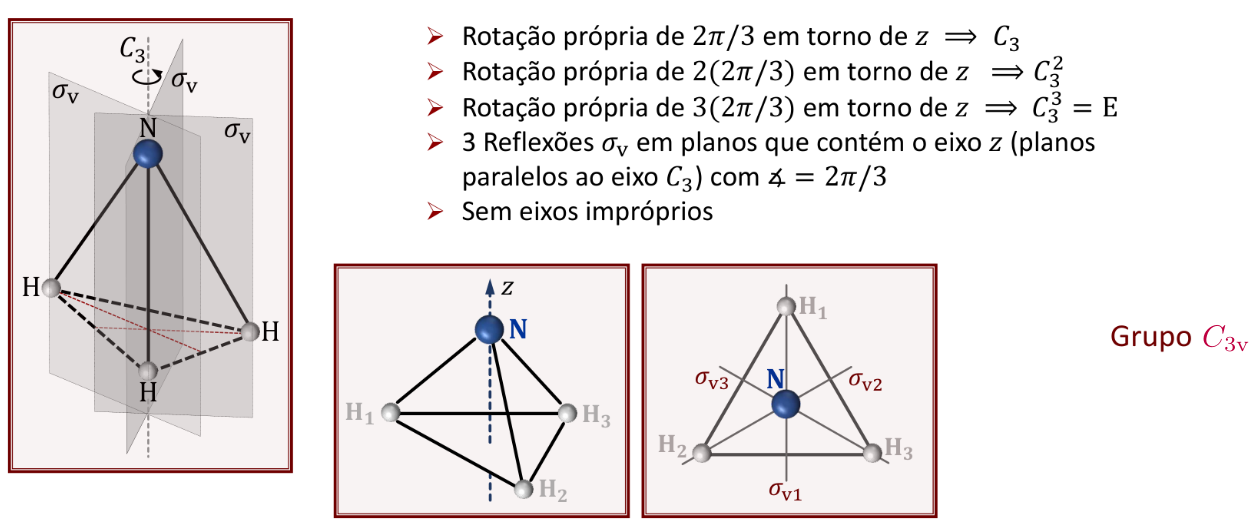
\includegraphics[width=\linewidth]{fig/C3v.png}
\caption{Grupo $C_{3\text{v}}$ associado à molécula de amônia.}
\label{fig:C3v}
\end{figure}

Nos slides da Aula 3 (Figura \ref{fig:C3v}), a professora deu como exemplo o grupo $C_{3\text{v}}$ da amônia. Este grupo contém 6 elementos, sendo eles
\begin{itemize}
\item a identidade $E$;
 \item as três reflexões $\sigma_{\text{v}1}$, $\sigma_{\text{v}2}$ e $\sigma_{\text{v}3}$ representadas na Figura \ref{fig:C3v};
\item as rotações $C_3$ (por $120^\circ)$ e $C_3^2$ (por $240^\circ$) pelo eixo que passa pelo átomo de nitrogênio N e o baricentro do triângulo definido pelos três átomos de hidrogênio H.
\end{itemize}

\begin{figure}[H]
\centering
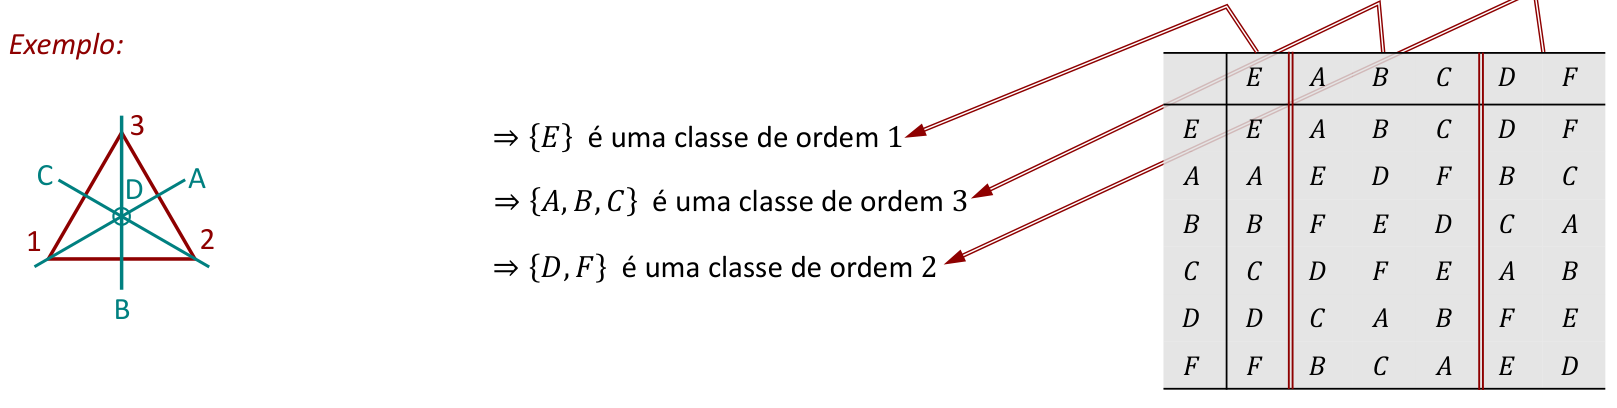
\includegraphics[width=\linewidth]{fig/triangulo.png}
\caption{Grupo do triângulo visto na Aula 2.}
\label{fig:triangulo}
\end{figure}

Nos slides da Aula 2 (Figura \ref{fig:triangulo}) a professora passou o grupo do triângulo. Note bem que se compararmos as Figuras \ref{fig:C3v} e \ref{fig:triangulo}, conseguimos estabelecer diretamente um isomorfismo entre o grupo do triângulo e o grupo $C_{3\text{v}}$. De fato, colocando os dois desenhos lado a lado na Figura \ref{fig:comp} vemos imediatamente a identificação:
\begin{equation} \label{eq:identificacao}
E \leftrightarrow E, \quad
\sigma_{\text{v}1} \leftrightarrow B, \quad
\sigma_{\text{v}2} \leftrightarrow A, \quad
\sigma_{\text{v}3} \leftrightarrow C, \quad
C_3 \leftrightarrow D, \quad
C_3^2 \leftrightarrow F.
\end{equation}

Devido a esse isomorfismo, todas as propriedades algébricas entre os grupos seram iguais, em particular a tabela de multiplicação e a partição do grupo em classes.

\begin{figure}[H]
\centering
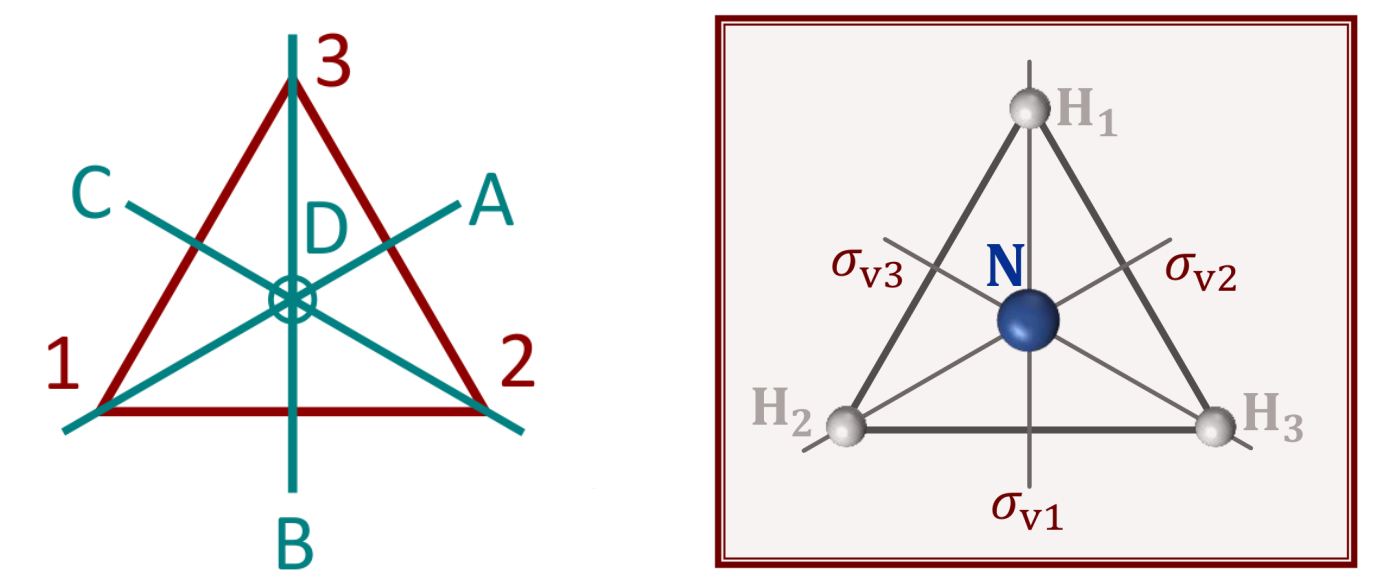
\includegraphics[width=0.6\linewidth]{fig/comp.png}
\caption{Identificação imediata entre os elementos do grupo do triângulo e o grupo $C_{3\text{v}}$.}
\label{fig:comp}
\end{figure}


\subsection*{1. Ordem}

O grupo se escreve $C_{3\text{v}} = \{E, \sigma_{\text{v}1}, \sigma_{\text{v}2}, \sigma_{\text{v}3}, C_3, C_3^2\}$ e possui ordem $6$.

\subsection*{2. Tabela de Multiplicação}

Pelo isomorfismo, a tabela de multiplicação do grupo $C_{3\text{v}}$ é idêntica ao do grupo do triângulo (mostrada na Figura \ref{fig:triangulo}), dado que façamos a identificação \ref{eq:identificacao}. Portanto ela é:

\begin{table}[ht]
\caption{Tabela de multiplicação do grupo $C_{3\text{v}}$, construída pela tabela de multiplicação do grupo do triângulo (Figura \ref{fig:triangulo}) e o isomorfismo da equação \ref{eq:identificacao}.}
\centering
\begin{tabular}{ |c|c c c c c c| }
\hline
\phantom{x}          & $E$                  & $\sigma_{\text{v}1}$   & $\sigma_{\text{v}2}$ & $\sigma_{\text{v}3}$ & $C_3$                & $C_3^2$ \\
\hline
$E$                  & $E$                  & $\sigma_{\text{v}1}$   & $\sigma_{\text{v}2}$ & $\sigma_{\text{v}3}$ & $C_3$                & $C_3^2$ \\
$\sigma_{\text{v}1}$ & $\sigma_{\text{v}1}$ & $E$                    & $C_3$                & $C_3^2$              & $\sigma_{\text{v}1}$ & $\sigma_{\text{v}3}$ \\
$\sigma_{\text{v}2}$ & $\sigma_{\text{v}2}$ & $C_3^2$                & $E$                  & $C_3$                & $\sigma_{\text{v}3}$ & $\sigma_{\text{v}2}$ \\
$\sigma_{\text{v}3}$ & $\sigma_{\text{v}3}$ & $C_3$                  & $C_3^2$              & $E$                  & $\sigma_{\text{v}2}$ & $\sigma_{\text{v}1}$ \\
$C_3$                & $C_3$                & $\sigma_{\text{v}3}$   & $\sigma_{\text{v}2}$ & $\sigma_{\text{v}1}$ & $C_3^2$              & $E$ \\
$C_3^2$              & $C_3^2$              & $\sigma_{\text{v}1}$   & $\sigma_{\text{v}3}$ & $\sigma_{\text{v}2}$ & $E$                  & $C_3$ \\
\hline
\end{tabular}
\label{tab:mult}
\end{table}

\subsection*{3. Cíclico?}

Como vemos na tabela de multiplicação \ref{tab:mult}, ela não é simétrica e portanto o grupo não é abeliano. Assim, ele também não é cíclico (não existe um único elemento gerador que gera todo o grupo).

\subsection*{4. Abeliano?}

A tabela de multiplicação \ref{tab:mult} não é simétrica, logo o grupo não é abeliano.

\subsection*{5. Classes}

As classes do grupo $C_{3\text{v}}$ são idênticas às classes do grupo do triângulo, ao realizarmos a identificação na equação \ref{eq:identificacao}. Portanto, olhando na Figura \ref{fig:triangulo} vemos que as três classes são $\{E\}$, $\{\sigma_{\text{v}1}, \sigma_{\text{v}2}, \sigma_{\text{v}3}\}$ e $\{C_3, C_3^2\}$.

\end{document}
